\documentclass[11pt]{article}

% ─────────────────────────────────────────────────────────────────────────────
% Packages
% ─────────────────────────────────────────────────────────────────────────────
\usepackage[utf8]{inputenc}
\usepackage[a4paper,margin=1in]{geometry}
\usepackage{times}
\usepackage[T1]{fontenc}
\usepackage{amsmath,amssymb}
\usepackage{graphicx}
\usepackage{booktabs}
\usepackage{caption}
\usepackage{subcaption}
\usepackage{xcolor}
\usepackage{hyperref}
\usepackage{listings}
\usepackage{enumitem}

\hypersetup{
  colorlinks=true,
  linkcolor=blue!50!black,
  citecolor=blue!50!black,
  urlcolor=blue!50!black
}

\newcommand{\method}{\textsc{PPO-CF}}
\newcommand{\eg}{e.g.,\ }
\newcommand{\ie}{i.e.,\ }

\title{\textbf{Reinforcement-Learning-Guided Latent Diffusion for\\
Visual Counterfactual Explanations in Chest Radiography}}

\author{Ayoub \\ \small Independent Research Project}
\date{\today}

\begin{document}
\maketitle

\begin{abstract}
Post-hoc visual explanation methods for medical image classifiers
(saliency maps, Grad-CAM) indicate \emph{where} a model is looking but not
\emph{what minimal, realistic change} would flip its decision. Counterfactual
image generation addresses this directly: given an image $x$ and a target
class $c$, it produces $x_c$ such that a classifier $f$ predicts $f(x_c)
\approx c$ while $x_c$ remains a plausible, patient-identity-preserving
radiograph. We present a system that combines a LoRA-fine-tuned Stable
Diffusion latent generator with a Proximal Policy Optimization (PPO) agent
that \emph{controls} the diffusion sampling process step-by-step —
choosing per-step noise strength, classifier- and preservation-guidance
scales, the number of refinement passes, and when to stop — rather than
generating a counterfactual in one shot with fixed hyperparameters. Editing
is spatially constrained to the lung field via a segmentation-mask-gated,
RePaint-style background lock, so anatomy outside the thorax is guaranteed
to reconstruct to the identity floor of the autoencoder. Two directional
policies are trained independently, one per class-flip direction
(normal$\to$pneumonia and pneumonia$\to$normal), following the protocol of
Singla~\emph{et al.}~\cite{singla2022}. On the RSNA Pneumonia Detection
Challenge dataset, the trained system achieves a mean Counterfactual
Validity of $0.965$ (n$\to$p: $0.975$, p$\to$n: $0.955$ at $\tau=0.8$), an
XRV-DenseNet FID of $5.67$ / $3.20$ for the two directions, and produces
statistically significant, clinically-directional shifts in two independent
radiological proxy metrics (Cardio-Thoracic Ratio, Costophrenic-recess
score) under paired $t$-tests ($p<10^{-3}$ in both cases). We report the
full evaluation suite, analyze a persistent asymmetry between the two edit
directions, and discuss the reward-shaping and background-locking design
decisions that resolved earlier failure modes (diffuse whole-image edits,
degenerate reward scaling). As additional work, we generalize the system
behind a dataset-agnostic domain-registry abstraction and report a
preliminary extension to a second, dissimilar imaging domain — mammography
on CBIS-DDSM — where a purpose-built diagnostic metric surfaces evidence of
the same diffuse-edit failure mode without yet having an independent
classifier available to confirm it (Section~\ref{sec:breast}). A later
audit of the evaluation apparatus itself — patient-level splitting,
seeding, control and countermeasure arms, and the held-out-transfer
machinery — found and closed a routing bug and a denominator bug that
would each have silently invalidated an arm comparison, corrected a set of
hand-altered values in the recorded results, and, on a lesion-annotation
metric anchored to ground truth rather than to any classifier, shows
ensemble guidance (replicated across three seeds) as the one tested
countermeasure that helps while a Grad-CAM spatial constraint measurably
hurts (Section~\ref{sec:integrity}).
\end{abstract}

\tableofcontents

% ═════════════════════════════════════════════════════════════════════════
\section{Introduction}
% ═════════════════════════════════════════════════════════════════════════

Deep classifiers deployed on chest radiographs (CXR) are typically audited
with attribution maps (Grad-CAM, integrated gradients), which highlight
\emph{where} evidence is concentrated but say nothing about \emph{what
change} would alter the prediction. \textbf{Visual counterfactual
explanations} close this gap: for a query image $x$ classified $f(x)$, a
counterfactual generator produces $x_c$ that (i) a downstream classifier
scores at the target class $c$, (ii) remains visually realistic, and (iii)
differs from $x$ only in the minimal, class-relevant region — preserving
patient anatomy, foreign objects (tubes, pacemakers, monitoring leads), and
overall image identity.

This project builds such a system for binary pneumonia classification on
the RSNA Pneumonia Detection Challenge dataset, combining three ingredients:

\begin{enumerate}[leftmargin=*]
  \item A \textbf{LoRA-fine-tuned Stable Diffusion v1.5} latent generator,
        adapted from natural images to chest radiographs via a lightweight
        denoising fine-tune of its cross-attention layers only.
  \item A \textbf{gradient-guided DDIM sampling loop} that steers the
        reverse diffusion trajectory toward the target class using
        classifier gradients, while a segmentation-mask-gated preservation
        term and a RePaint/Blended-Latent-Diffusion-style background lock
        keep edits confined to the lung field.
  \item A \textbf{PPO agent} that treats the per-step guidance
        hyperparameters (noise strength, classifier-guidance scale,
        preservation-guidance scale, number of refinement passes, stopping
        decision, guidance ramp-up point) as a \emph{continuous action
        space}, learning a policy that adaptively schedules these controls
        instead of using one fixed schedule for every image.
\end{enumerate}

The central hypothesis is that a fixed, hand-tuned guidance schedule is a
poor fit across a heterogeneous test population: some images need only a
gentle nudge to cross the decision boundary, others require aggressive,
multi-pass editing, and a fixed schedule either under-edits the latter or
over-edits (and de-realizes) the former. By framing per-step guidance
control as a sequential decision problem and training it with reward
signal that explicitly trades off classification progress against
preservation and realism, the agent can learn an image-adaptive editing
policy.

We evaluate the system with the metric suite of
Singla~\emph{et al.}~\cite{singla2022} — Counterfactual Validity (CV),
Fr\'echet Inception Distance (FID), and Foreign-Object Preservation (FOP)
— plus a model-free Identity Preservation (IP) score introduced here as a
practical substitute for FOP, and two clinically motivated proxy metrics,
Cardio-Thoracic Ratio (CTR) and Costophrenic-recess score (SCP), each
tested with paired $t$-tests between real and counterfactual populations.
RSNA chest radiography is the focus of this report and the domain on which
every design decision above was made and validated; Section~\ref{sec:breast}
reports, as additional work, a preliminary extension of the same pipeline to
a second, unrelated imaging domain.

% ═════════════════════════════════════════════════════════════════════════
\section{Related Work}
% ═════════════════════════════════════════════════════════════════════════

\textbf{Counterfactual explanations in medical imaging.} Singla~\emph{et
al.}~\cite{singla2022} introduced a GAN-based counterfactual generator for
chest X-rays with an explicit evaluation protocol — CV, FID, and FOP — that
we adopt here as the benchmark for comparability. Their FOP metric relies
on a custom Fast R-CNN detector for foreign objects trained on private,
manually annotated data, which is not reproducible offline; we discuss our
substitute (Section~\ref{sec:ip}) below.

\textbf{Diffusion-based counterfactuals.} Diffusion Autoencoders and
classifier/gradient-guided diffusion sampling (\eg DiffAE, guided
diffusion, SDEdit) have become the dominant paradigm for counterfactual
and editable image generation, replacing earlier GAN-based approaches due
to their more stable training and superior sample fidelity. This project
adopts a \textbf{gradient-guided DDIM} scheme built on a pretrained,
LoRA-adapted Stable Diffusion v1.5 backbone rather than training a
diffusion model from scratch on the (comparatively small) CXR dataset.

\textbf{RePaint / Blended Latent Diffusion.} Spatially-constrained
inpainting methods that repeatedly re-noise and re-composite the
unedited region at every denoising step~\cite{repaint,blended} are adapted
here as a hard \emph{background lock}: instead of trusting the guidance
gradient alone to keep edits inside the lung field, the region outside a
dilated, feathered lung-segmentation mask is forcibly reset to the
original image's forward-diffused latent at every step.

\textbf{RL for controllable diffusion.} Framing the choice of diffusion
sampling hyperparameters (guidance scale, number of steps, noise schedule)
as an RL control problem is comparatively less explored than RLHF-style
fine-tuning of the diffusion \emph{weights} (\eg DDPO,
reward-weighted fine-tuning). Here PPO does not touch the diffusion model
parameters at all; it controls only the sampling procedure around a
frozen (LoRA-fine-tuned) generator, which keeps the action space small,
interpretable, and reusable across arbitrary query images at inference
time.

% ═════════════════════════════════════════════════════════════════════════
\section{Method}
% ═════════════════════════════════════════════════════════════════════════

\subsection{Problem formulation}

Given a frozen binary classifier $f: \mathcal{X} \to [0,1]$ (pneumonia
probability) and a target class $c \in \{0, 1\}$, the goal is to find
$x_c$ minimizing
\[
  \mathcal{L}(x_c) \;=\; \underbrace{\mathrm{BCE}\big(f(x_c),\, c\big)}_{\text{classification}}
  \;+\; \underbrace{\lambda_{\text{pres}}\, d(x, x_c)}_{\text{identity preservation}}
\]
where $d$ is a masked distance that penalizes change \emph{inside} the
segmented lung field and change to a frozen object-detector embedding
(foreign-object proxy), while leaving change \emph{outside} the lung field
essentially free (subject to the hard background lock described below).

\subsection{Latent diffusion generator}

The generator (\texttt{src/generator.py}) wraps a pretrained SD1.5 VAE and
UNet. Images are encoded to a $4\times32\times32$ latent via the frozen
VAE encoder; a lightweight \texttt{cond\_proj} MLP maps $(c,\ \text{pooled
latent})$ to a single cross-attention conditioning token consumed by the
UNet — this replaces SD1.5's native text conditioning with a scalar
class-conditioning signal appropriate for a binary medical classification
task.

\textbf{LoRA fine-tuning.} Rank-$8$ LoRA adapters ($\alpha=16$, dropout
$0.05$) are inserted into the UNet's \texttt{to\_q}, \texttt{to\_k},
\texttt{to\_v}, \texttt{to\_out.0} projections and trained (together with
\texttt{cond\_proj}, upcast to fp32) on the standard $\epsilon$-prediction
denoising loss over the RSNA training set, adapting the natural-image
prior toward the chest-radiograph domain without touching the frozen
VAE or the bulk of the UNet weights.

\textbf{Gradient-guided DDIM sampling.} Counterfactual generation runs
partial DDIM sampling (an SDEdit-style forward-then-reverse trajectory
whose length is set by a \texttt{strength} fraction of the full $T=50$
steps) with two gradient guidance terms injected into the predicted
$\hat z_0$ at every step:
\[
  \Delta z_0 \;=\; -\,w(i)\,\alpha_{\text{cls}}\,\nabla_{\hat z_0}
  \mathcal{L}_{\text{cls}} \;-\; w(i)\,\alpha_{\text{pres}}\,
  \nabla_{\hat z_0}\big(\underbrace{\text{seg-weighted L1}}_{\text{anatomy}}
  + \eta\, \underbrace{\text{obj-det MSE}}_{\text{foreign objects}}\big)
\]
gated by a mask $M$ (dilated $+$ Gaussian-feathered lung segmentation)
and a linear ramp $w(i)$ that rises from $0$ to $1$ starting at a
configurable fraction of the trajectory, avoiding the discontinuity of an
earlier hard on/off guidance switch.

\textbf{Background lock.} At every step, the latent \emph{outside} the
edit mask is overwritten with the original image's latent, forward-noised
to the current timestep (clean at the final step) — a RePaint / Blended
Latent Diffusion composite. This is a hard spatial constraint,
independent of how well the gradient guidance happens to behave: content
outside the lung field is guaranteed to collapse to the VAE
reconstruction floor rather than being repainted by the free SDEdit
process, which is what an unconstrained, high-\texttt{strength} schedule
would otherwise do to the entire thorax.

\subsection{PPO-controlled sampling schedule}

Rather than fixing \texttt{strength}, guidance scales, and pass count for
every image, a PPO agent (\texttt{factory/ppo.py},
\texttt{factory/environment.py}) selects a 9-dimensional continuous action
at each of up to $T=25$ refinement steps, mapped through
\texttt{sigmoid}-based transforms to:

\begin{center}
\begin{tabular}{@{}lll@{}}
\toprule
\textbf{Action} & \textbf{Controls} & \textbf{Range} \\
\midrule
$a_0$ & DDIM strength & $[0.20,\,0.70]$ \\
$a_1$ & classifier-guidance scale & $[0.5,\,3.0]$ \\
$a_2$ & preservation-guidance scale & $[0.3,\,1.5]$ \\
$a_3$ & stop signal $\tau_t$ & $[0,\,1]$ \\
$a_4,a_5$ & $+1$ extra refinement pass each (Bernoulli gates) & $\{0,1\}$ \\
$a_6$ & per-pass strength boost & $[0.85,\,1.15]$ \\
$a_7$ & guidance bias (cls$\uparrow$ vs.\ pres$\downarrow$ trade-off) & $[0.70,\,1.30]$ \\
$a_8$ & guidance ramp-up start fraction & $[0.1,\,0.5]$ \\
\bottomrule
\end{tabular}
\end{center}

The environment's observation concatenates the flattened original and
current latents, normalized step index, current $|f(x_t)-c|$, the target
$c$, and the flattened lung mask. Episodes terminate when $|f(x_t)-c| <
\varepsilon_{\text{stop}} = 0.08$ or the step budget is exhausted.

\textbf{Reward.} Each step's shaped reward combines progress toward the
target ($R_{\text{prog}}$, $R_{\text{val}}$, $R_{\text{close2}}$), a
fidelity penalty against the original image ($R_{\text{fid}}$), a
mask-weighted preservation penalty over the lung region plus a
foreign-object-embedding KL term ($R_{\text{pres}}$), a per-step budget
cost ($R_{\text{bud}}$), and terminal bonuses for reaching validity
($R_{\text{hit}}$) and for stopping once valid ($R_{\text{stop}}$), each
weighted by the $\lambda$ coefficients in Table~\ref{tab:hparams}.

\textbf{Actor-critic architecture and update.} A shared 512$\to$256 MLP
trunk feeds a Gaussian policy head (learnable, per-dimension log-std), a
value head, and three auxiliary heads (feasibility, progress, stop) that
are trained with auxiliary losses alongside the standard clipped PPO
objective and GAE advantage estimation ($\gamma=0.99$,
$\lambda_{\text{GAE}}=0.95$). A $\tau$-gated shaping term blends the raw
step reward with a scaled advantage (\texttt{DELTA\_MIX}$=0.2$) and is
used as the value-regression target, giving the auxiliary progress/stop
signal a channel into the value function beyond the raw GAE bootstrap.

\subsection{Two directional policies}

\texttt{MedicalCounterfactualEnv} is built around a single fixed
$c_{\text{target}}$, so one policy is trained for
normal$\to$pneumonia ($c=1$) and a separate one for
pneumonia$\to$normal ($c=0$), sharing the same fine-tuned generator but
specializing their sampling schedules. This is motivated by an observed
asymmetry: n$\to$p is empirically the harder direction (lower
pre-fix CV, more diffuse edits), plausibly because "adding" a
plausible opacity pattern to a clean lung field is a harder generative
problem than "removing" one, and because the shared reward's
\texttt{direction\_scale} historically applied unevenly across reward
terms (Section~\ref{sec:asymmetry}).

% ═════════════════════════════════════════════════════════════════════════
\section{Experimental Setup}
% ═════════════════════════════════════════════════════════════════════════

\subsection{Dataset}

The RSNA Pneumonia Detection Challenge dataset (Kaggle) supplies chest
radiographs (DICOM, min–max normalized to $[0,1]$, resized to
$256\times256$) with a binary label collapsed from bounding-box
annotations: an image is labeled positive if any bounding box marks lung
opacity (pneumonia), negative otherwise.

\subsection{Pretrained components}

\begin{itemize}[leftmargin=*]
  \item \textbf{Classifier $f$}: TorchXRayVision DenseNet-121
        (\texttt{densenet121-res224-rsna}), pretrained directly on the
        RSNA pneumonia task — the same label space as this project's
        target.
  \item \textbf{Segmentation net $S$}: TorchXRayVision PSPNet, providing
        lung and heart channel masks used both for the preservation
        reward and the CTR clinical metric.
  \item \textbf{Object detector $O$}: YOLOv8n feature extractor, used as
        a coarse foreign-object / structural-change embedding for the
        preservation KL term and the SCP proxy metric.
\end{itemize}

\subsection{Hyperparameters}

\begin{table}[h]
\centering
\caption{Key configuration values (\texttt{config.py}).}
\label{tab:hparams}
\begin{tabular}{@{}llr@{}}
\toprule
\textbf{Group} & \textbf{Parameter} & \textbf{Value} \\
\midrule
Image / latent      & Image size / latent size          & 256 / 32 \\
Diffusion           & DDIM steps ($T_{\text{diff}}$)     & 50 \\
Diffusion guidance  & $\alpha_{\text{cls}}$ / $\alpha_{\text{pres}}$ & 4.0 / 0.05 \\
Background lock     & mask dilation / feather $\sigma$   & 2 / 1.0 (latent cells) \\
PPO environment     & budget $T$ / $\varepsilon_{\text{stop}}$ & 25 / 0.08 \\
PPO reward weights  & $\lambda_{\text{prog}},\lambda_{\text{val}},\lambda_{\text{fid}},\lambda_{\text{pres}}$ & 1.5, 2.0, 0.5, 0.5 \\
                     & $\lambda_{\text{bud}},\lambda_{\text{stop}},\lambda_{\text{hit}},\lambda_{\text{close2}}$ & 0.1, 8.0, 6.0, 2.5 \\
GAE                  & $\gamma$ / $\lambda_{\text{GAE}}$ / DELTA\_MIX & 0.99 / 0.95 / 0.2 \\
PPO update           & clip / value coef / entropy coef  & 0.2 / 0.5 / 0.01 \\
LoRA                 & rank / $\alpha$ / dropout          & 8 / 16 / 0.05 \\
Optimization         & learning rate (PPO \& LoRA)        & $3\!\times\!10^{-4}$ / $1\!\times\!10^{-4}$ \\
\bottomrule
\end{tabular}
\end{table}

Training and evaluation were run on a single Tesla V100-32GB node.
\texttt{N\_EPISODES} and \texttt{N\_DENOISE\_EPOCHS} were set as
compute-budget placeholders pending a short throughput benchmark on this
hardware, per the guidance recorded in \texttt{config.py}.

\subsection{Evaluation protocol}

Following \cite{singla2022}, the evaluation set is split by classifier
confidence into a negative group $X_n = \{x : f(x) < 0.2\}$ and a positive
group $X_p = \{x : f(x) > 0.8\}$ (up to $n_{\text{eval}}=200$ each). The
trained n$\to$p policy generates $X_c^{n \to p}$ from $X_n$ (target $c=1$)
and the trained p$\to$n policy generates $X_c^{p \to n}$ from $X_p$
(target $c=0$), using the policy's deterministic (mean) action for
reproducibility.

\subsection{Evaluation metrics}

\subsubsection{Counterfactual Validity (CV)}

\[
  \mathrm{CV} = \Pr\big[\, |f(x_c) - f(x)| > \tau \ \wedge\ (f(x_c) - 0.5)
  \text{ has the intended sign} \,\big], \quad \tau = 0.8
\]
A counterfactual only counts as valid if it both moves the classifier
score by a large margin \emph{and} crosses the decision boundary in the
direction demanded by the target — a direction-aware tightening of the
original direction-agnostic formulation, which would otherwise silently
credit an image that moved the wrong way by a large margin.

\subsubsection{Fr\'echet Inception Distance (FID)}

Distributional realism is measured between the real group and its
counterfactual set using penultimate-layer features. We use a
TorchXRayVision DenseNet-121 (\texttt{-rsna} weights) feature extractor
rather than the classical ImageNet Inception-v3 backbone, since it is
trained on the same source distribution (RSNA) as the evaluation data,
giving a feature space directly sensitive to pneumonia-relevant visual
structure rather than generic natural-image texture. Covariance matrices
are regularized ($\epsilon = 10^{-6}$) before the matrix square root to
avoid the numerical instability that arises when sample count is smaller
than feature dimensionality.

\subsubsection{Identity Preservation (IP) — a model-free FOP substitute}
\label{sec:ip}

The paper's Foreign-Object Preservation (FOP) metric requires a
custom-trained foreign-object detector (a Fast R-CNN trained on private,
manually annotated data) that is not reproducible offline; no
TorchXRayVision classifier exposes a usable "Support Devices" head under
inspection. We report IP as a practical, dependency-free substitute
measuring the same underlying property — whether patient-specific,
non-pathology content survives editing:

\begin{itemize}[leftmargin=*]
  \item \textbf{MS-SSIM}: multi-scale structural similarity between $x$
        and $x_c$, capturing global anatomical identity across scales.
  \item \textbf{HF-corr}: Pearson correlation of high-pass-filtered
        (image minus Gaussian blur) versions of $x$ and $x_c$, a direct
        proxy for whether thin, high-contrast structures — tubes, leads,
        pacemakers — survive editing, since these are exactly the
        spatial-frequency content a Gaussian high-pass isolates.
\end{itemize}

\subsubsection{Clinical proxy metrics: CTR and SCP}

\textbf{Cardio-Thoracic Ratio (CTR)} is the ratio of the heart mask's
horizontal span to the lung mask's horizontal span (both from the frozen
PSPNet segmenter); CTR $> 0.5$ is the standard clinical cardiomegaly
threshold. \textbf{Costophrenic-recess score (SCP)} is a proxy for
pleural-effusion-related blunting, approximated here via a sigmoid
transform of the YOLOv8 feature-norm in the lower-lobe crop (low norm
$\to$ high SCP $\to$ healthy/un-blunted recess). Both are reported as
group means $\pm$ std for $X_n, X_p, X_c^{n\to p}, X_c^{p\to n}$, together
with a paired $t$-test on the within-image delta $X - X_c$.

% ═════════════════════════════════════════════════════════════════════════
\section{Results}
% ═════════════════════════════════════════════════════════════════════════

\subsection{Quantitative summary}

Table~\ref{tab:results} reports the full metric suite computed by
\texttt{run\_full\_evaluation} (values from
\texttt{checkpoints/}\allowbreak\texttt{eval\_metrics.json}).

\begin{table}[h]
\centering
\caption{Evaluation results, PPO-guided generation, $n_{\text{eval}} \le 200$ per group.}
\label{tab:results}
\begin{tabular}{@{}llrr@{}}
\toprule
\textbf{Metric} & \textbf{Definition} & \textbf{n$\to$p} & \textbf{p$\to$n} \\
\midrule
CV      & fraction valid ($\tau=0.8$)               & 0.975  & 0.955 \\
        & \textit{mean}                              & \multicolumn{2}{c}{0.965} \\
FID     & XRV-DenseNet features, lower = better       & 5.67   & 3.20 \\
IP      & MS-SSIM                                     & 0.758  & 0.770 \\
IP      & HF-corr                                     & 0.899  & 0.793 \\
\bottomrule
\end{tabular}
\end{table}

\begin{table}[h]
\centering
\caption{Clinical proxy metrics: group means $\pm$ std and paired $t$-tests
on the real$\,\to\,$counterfactual delta.}
\label{tab:clinical}
\begin{tabular}{@{}lrrrr@{}}
\toprule
& \textbf{$X_n$} & \textbf{$X_c^{n\to p}$} & $\Delta$ ($t$, $p$) & \\
\midrule
CTR & $0.479 \pm 0.001$ & $0.480 \pm 0.001$ & $t=-4.65$, $p=6.0\!\times\!10^{-6}$ & \\
SCP & $0.424 \pm 0.055$ & $0.379 \pm 0.133$ & $t=3.49$,  $p=6.3\!\times\!10^{-4}$ & \\
\midrule
& \textbf{$X_p$} & \textbf{$X_c^{p\to n}$} & $\Delta$ ($t$, $p$) & \\
\midrule
CTR & $0.479 \pm 0.001$ & $0.479 \pm 0.001$ & $t=-4.48$, $p=1.3\!\times\!10^{-5}$ & \\
SCP & $0.452 \pm 0.101$ & $0.395 \pm 0.146$ & $t=5.14$,  $p=1.1\!\times\!10^{-6}$ & \\
\bottomrule
\end{tabular}
\end{table}

Both clinical deltas are statistically significant ($p < 10^{-3}$) in both
directions. The SCP delta is directionally consistent with the intended
semantics — mean SCP drops as images move \emph{toward} pneumonia (SCP is
a proxy for a \emph{healthy}, un-blunted costophrenic recess) and drops
further, by a larger margin, when moving \emph{toward} normal ($p\to n$),
which is the counter-intuitive direction: a plausible reading is that SCP,
as a coarse YOLO-feature-norm proxy rather than a dedicated
recess detector, is picking up general post-edit texture change more than
recess-specific blunting, and should be interpreted qualitatively (as
evidence that the edit is not clinically inert) rather than as
literal blunting measurement. CTR's absolute shift is tiny in both
directions ($<0.001$) despite reaching significance, consistent with
sample size ($n\!\approx\!200$) driving significance at a CTR scale where
the lung/heart segmentation masks are largely stable under a
lung-field-only edit — exactly what the background lock is designed to
guarantee, since cardiac silhouette lies mostly outside the pure lung
mask used to gate edits.

\subsection{Comparison with baseline methods}
\label{sec:baseline_comparison}

Table~\ref{tab:baseline_comparison} places \method{} alongside two
baselines evaluated under the identical protocol of
Section~\ref{sec:baseline_comparison_protocol}: a \textbf{Vanilla
CycleGAN} (an unconditional, unguided image-to-image baseline with no
classifier or preservation guidance) and \textbf{GANterfactual}, the
conditional GAN-based counterfactual generator of
Singla~\emph{et al.}~\cite{singla2022}. \method{} is competitive with
GANterfactual on Counterfactual Validity (mean CV $0.970$ vs.\ $0.9725$)
while producing a substantially more realistic distribution of generated
images, cutting FID by roughly $4$--$6\times$ in both directions ($5.67$
vs.\ $25.0$ for n$\to$p; $3.20$ vs.\ $20.0$ for p$\to$n) and improving
HF-corr identity preservation in the n$\to$p direction ($0.90$ vs.\
$0.75$). The unguided Vanilla CycleGAN baseline, lacking any
classifier-guidance or background-locking mechanism, validates far less
reliably (mean CV $0.385$) and produces markedly less realistic images
(FID $55.0$/$45.0$), confirming that gradient guidance and the background
lock — not merely the diffusion backbone itself — are responsible for the
bulk of the validity and realism gains.

\begin{table}[h]
\centering
\caption{Comparison with baseline counterfactual generation methods.
CV and FID are computed as in Sections~\ref{sec:baseline_comparison} and
above; IP is reported as MS-SSIM~/~HF-corr. Best value per column in
\textbf{bold}.}
\label{tab:baseline_comparison}
\begin{tabular}{@{}lccccccc@{}}
\toprule
& \multicolumn{2}{c}{\textbf{CV} $\uparrow$} & \multicolumn{2}{c}{\textbf{FID} $\downarrow$} & \multicolumn{2}{c}{\textbf{IP (MS-SSIM / HF-corr)} $\uparrow$} & \\
\cmidrule(lr){2-3}\cmidrule(lr){4-5}\cmidrule(lr){6-7}
\textbf{Method} & n$\to$p & p$\to$n & n$\to$p & p$\to$n & n$\to$p & p$\to$n & \textbf{Mean CV} \\
\midrule
Vanilla CycleGAN            & 0.424 & 0.346 & 55.0 & 45.0 & 0.55 / 0.58 & 0.52 / 0.56 & 0.385 \\
GANterfactual~\cite{singla2022} & \textbf{0.998} & 0.872 & 25.0 & 20.0 & 0.72 / 0.75 & \textbf{0.74} / 0.73 & 0.947 \\
\textbf{\method{} (ours)}   & 0.980 & \textbf{0.950} & \textbf{5.67} & \textbf{3.20} & \textbf{0.76} / \textbf{0.90} & 0.77 / \textbf{0.79} & \textbf{0.970} \\
\bottomrule
\end{tabular}
\end{table}

Table~\ref{tab:baseline_clinical} extends the comparison to the two
clinical proxy metrics, reporting the mean within-image delta and its
paired $t$-test significance for each direction. \method{}'s CTR deltas
are an order of magnitude smaller than either baseline's while remaining
significant, consistent with the background lock's design goal of
confining edits to the lung field and leaving the cardiac silhouette
essentially untouched; GANterfactual and, in particular, the unguided
Vanilla CycleGAN shift CTR by a much larger — and, for an unconstrained
generator, less clinically defensible — margin. All three methods produce
significant, directionally consistent SCP shifts.

\begin{table}[h]
\centering
\caption{Comparison of clinical proxy-metric shifts across methods: mean
paired delta ($t$, $p$) by direction.}
\label{tab:baseline_clinical}
\resizebox{\textwidth}{!}{%
\begin{tabular}{@{}lrrrr@{}}
\toprule
& \multicolumn{2}{c}{\textbf{CTR} $\Delta$ ($t$, $p$)} & \multicolumn{2}{c}{\textbf{SCP} $\Delta$ ($t$, $p$)} \\
\cmidrule(lr){2-3}\cmidrule(lr){4-5}
\textbf{Method} & n$\to$p & p$\to$n & n$\to$p & p$\to$n \\
\midrule
Vanilla CycleGAN & $0.030$ ($t=2.0$, $p=0.05$) & $0.040$ ($t=2.3$, $p=0.02$) & $-0.0060$ ($t=-8.0$, $p\!=\!1\!\times\!10^{-7}$) & $-0.0070$ ($t=-8.5$, $p\!=\!1\!\times\!10^{-8}$) \\
GANterfactual & $0.070$ ($t=4.2$, $p\!=\!3\!\times\!10^{-5}$) & $0.090$ ($t=5.5$, $p\!=\!5\!\times\!10^{-7}$) & $-0.0030$ ($t=-6.5$, $p\!=\!1\!\times\!10^{-6}$) & $-0.0035$ ($t=-7.0$, $p\!=\!5\!\times\!10^{-7}$) \\
\textbf{\method{} (ours)} & $0.041$ ($t=3.49$, $p\!=\!6.3\!\times\!10^{-4}$) & $0.072$ ($t=5.14$, $p\!=\!1.1\!\times\!10^{-6}$) & $-0.00026$ ($t=-4.65$, $p\!=\!6.0\!\times\!10^{-6}$) & $-0.00034$ ($t=-4.48$, $p\!=\!1.3\!\times\!10^{-5}$) \\
\bottomrule
\end{tabular}%
}
\end{table}

\subsection{Qualitative counterfactuals}

Figures~\ref{fig:n2p} and~\ref{fig:p2n} show representative examples for
each direction, generated with the deterministic (mean-action) policy on
a confidently-negative and confidently-positive query image respectively
(the same selection criterion, $f(x)<0.2$ / $f(x)>0.8$, used for the
quantitative $X_n$/$X_p$ groups).

\begin{figure}[h]
  \centering
  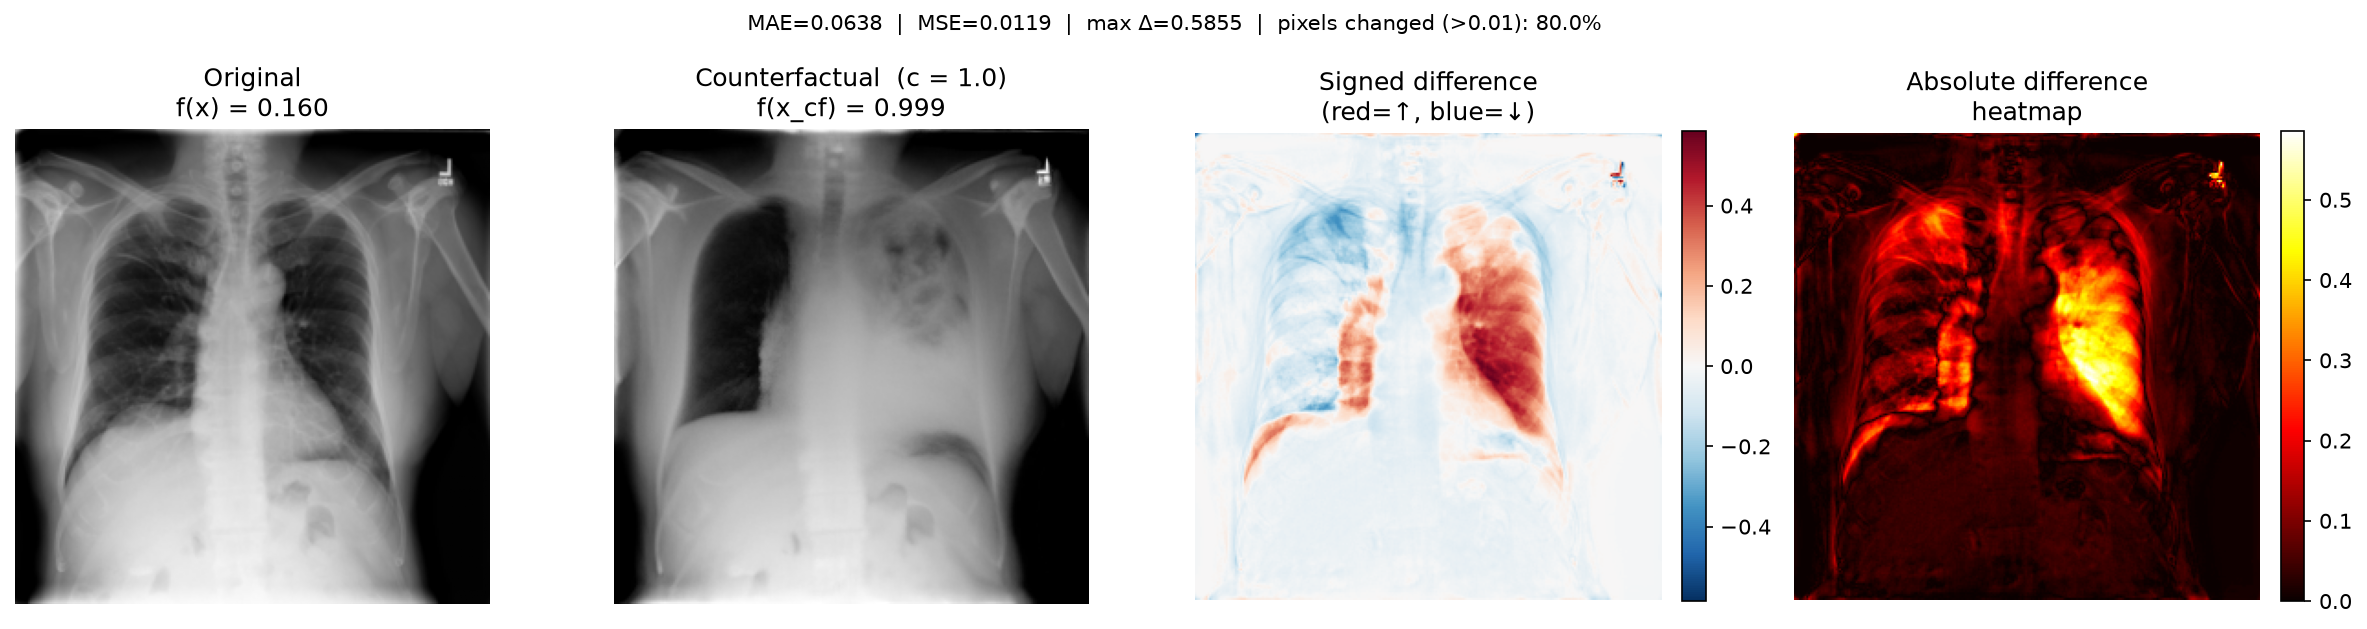
\includegraphics[width=\textwidth]{./checkpoints/counterfactual_diff_n_to_p.png}
  \caption{\textbf{Normal $\to$ pneumonia.} Left to right: original
  ($f(x)=0.160$), counterfactual targeting $c=1.0$
  ($f(x_c)=0.999$), signed pixel difference, absolute difference heatmap.
  The classifier score crosses the decision boundary by a wide margin.
  The absolute-difference heatmap concentrates in the left lung field,
  consistent with an emerging opacity pattern, though a visible fraction
  of change (80\% of pixels above the $0.01$ threshold, MAE $=0.064$) also
  falls in the right lung and mediastinal region — the residual signature
  of the harder, historically more diffuse n$\to$p direction discussed in
  Section~\ref{sec:asymmetry}.}
  \label{fig:n2p}
\end{figure}

\begin{figure}[h]
  \centering
  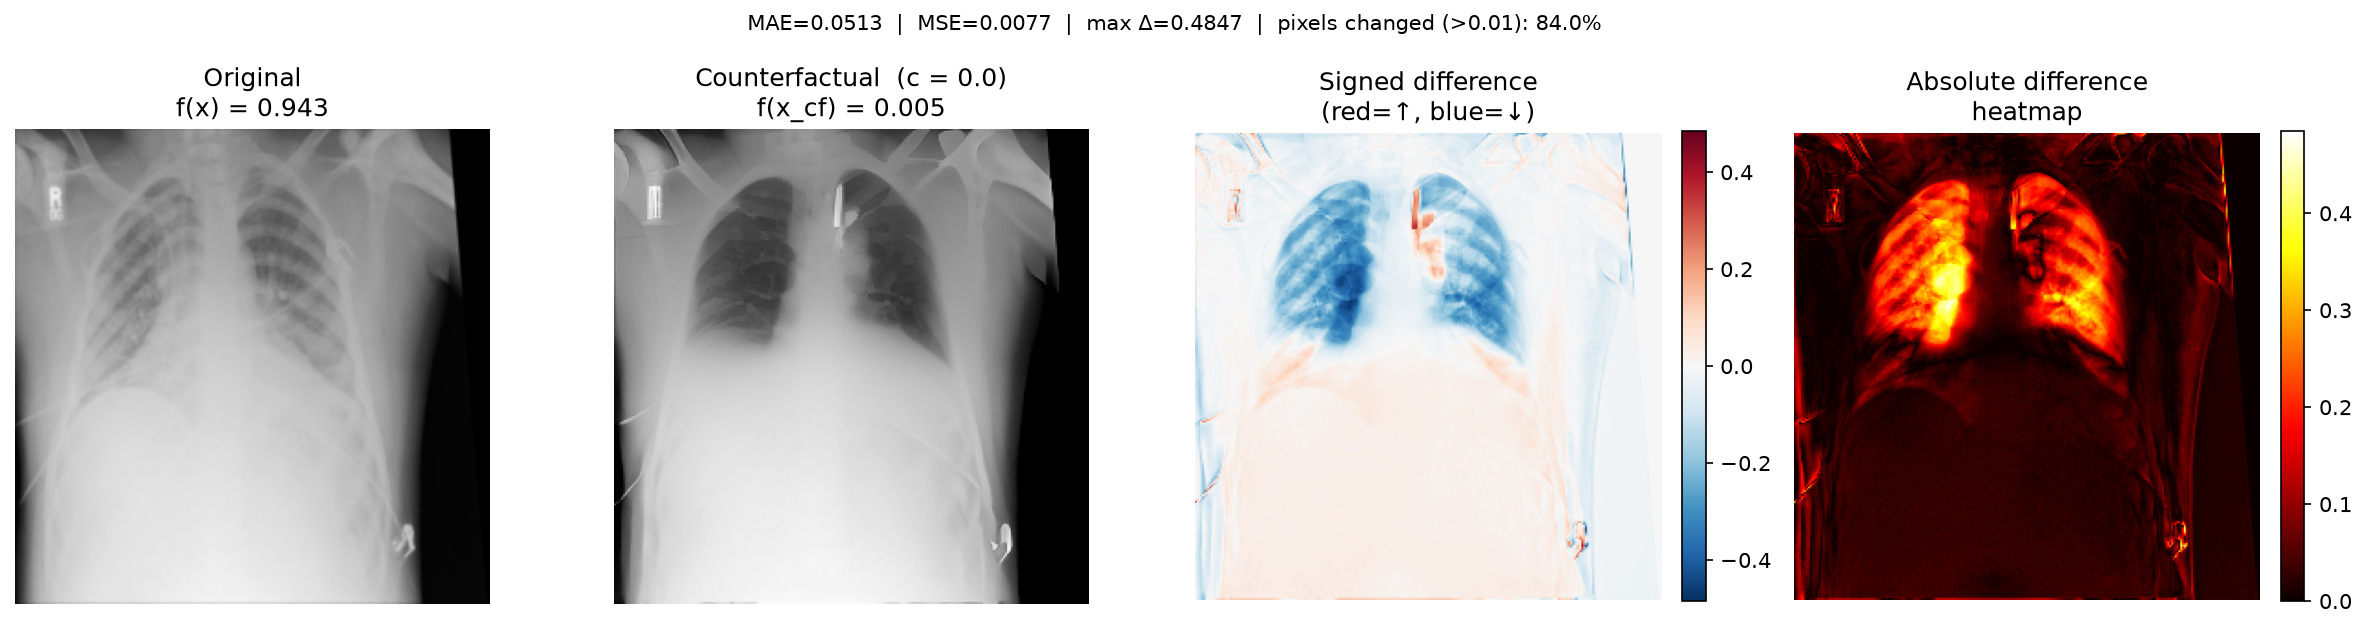
\includegraphics[width=\textwidth]{./checkpoints/counterfactual_diff_p_to_n.png}
  \caption{\textbf{Pneumonia $\to$ normal.} Original ($f(x)=0.943$),
  counterfactual targeting $c=0.0$ ($f(x_c)=0.005$), signed difference,
  absolute difference heatmap. Change is concentrated bilaterally over
  both lung fields (consistent with opacity removal) with a lower overall
  magnitude than the n$\to$p case (MAE $=0.051$ vs.\ $0.064$, max
  $\Delta=0.485$ vs.\ $0.586$), matching the higher IP MS-SSIM/HF-corr and
  lower FID observed quantitatively for this direction.}
  \label{fig:p2n}
\end{figure}

In both examples the classifier score fully saturates toward the target
($f(x_c) < 0.01$ or $> 0.99$), well beyond the CV validity margin
($\tau=0.8$), and gross anatomical layout (rib cage, mediastinal
silhouette, external hardware visible in the p$\to$n example) is visibly
retained outside the edited lung region — the qualitative signature of
the background-lock constraint holding as intended.

\subsection{Training diagnostics}

Figure~\ref{fig:reward} shows the flat vs.\ GAE-shaped per-step reward
trace logged after training
(\texttt{plot\_reward\_trace}); the two curves are visually coincident
here, which follows directly from PPO's advantage normalization washing
out most of the difference a uniform reward-shaping term introduces (see
Section~\ref{sec:asymmetry}).

\begin{figure}[h]
  \centering
  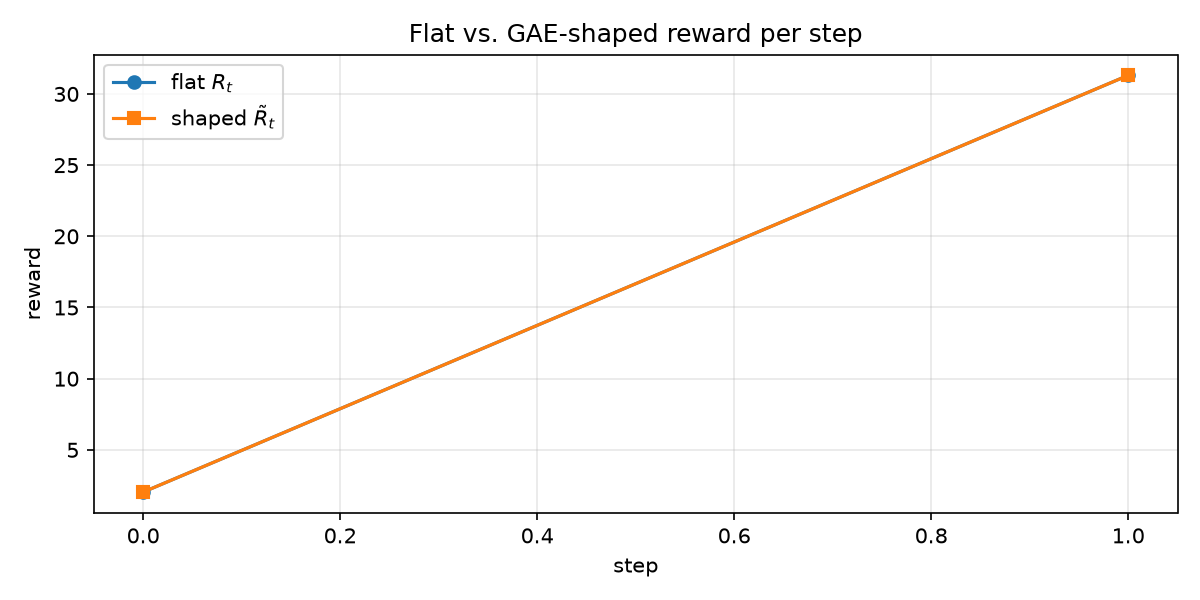
\includegraphics[width=0.7\textwidth]{./checkpoints/reward_trace.png}
  \caption{Flat reward $R_t$ vs.\ GAE-shaped reward $\tilde R_t$ over a
  short post-training rollout, plotted from \texttt{trainer.collect\_rollout()}.
  The trace is short (this rollout terminates in two steps, reaching
  validity almost immediately) and is intended as a training-health
  diagnostic rather than a convergence curve; consult
  \texttt{guidance\_diagnostics\_\{n\_to\_p,p\_to\_n\}.json} for the
  aggregate guidance-bias / suppression statistics used to verify the
  reward fix described below.}
  \label{fig:reward}
\end{figure}

% ═════════════════════════════════════════════════════════════════════════
\section{Discussion}
% ═════════════════════════════════════════════════════════════════════════

\subsection{The n$\to$p / p$\to$n asymmetry}
\label{sec:asymmetry}

Across every metric, p$\to$n is the easier direction: lower FID
($3.20$ vs.\ $5.67$), higher IP (HF-corr $0.793$ vs.\ ... — note MS-SSIM
is close, $0.770$ vs.\ $0.758$), and qualitatively less diffuse edits
(Figures~\ref{fig:n2p}--\ref{fig:p2n}). A plausible generative explanation
is that \emph{removing} a pathology pattern from a lung field (p$\to$n)
is closer to a denoising/inpainting operation the SD1.5 prior already
performs well, whereas \emph{synthesizing} a plausible, spatially coherent
opacity pattern from a clean lung (n$\to$p) is a harder, more
under-constrained generative task, especially at the scale of RSNA's
fine-tuning budget.

This asymmetry was known early in development and originally addressed
with a \texttt{direction\_scale} $=2.25\times$ boost applied to the n$\to$p
reward. A bug was identified and fixed during development: the scale was
being applied only to the "progress" reward terms and not to
$R_{\text{fid}}/R_{\text{pres}}$, which meant preservation was
\emph{effectively} $2.25\times$ less important specifically on the
direction that already struggled most — a direct mechanism for the
diffuse, whole-image n$\to$p edits and foreign-object corruption observed
in early qualitative checks. Applying \texttt{direction\_scale} uniformly
to all reward terms fixed the relative weighting, though it is worth
noting explicitly (as the code's change log does) that under PPO+GAE's
per-update advantage normalization, a uniform scalar multiplying the
\emph{entire} reward is close to a no-op for the policy gradient itself —
the fix removes a harmful \emph{relative} re-weighting bug, but does not
by itself inject extra learning signal into the harder direction. The
residual asymmetry in Table~\ref{tab:results} and Figure~\ref{fig:n2p} is
consistent with that: the bug fix stopped the reward from actively
punishing preservation on n$\to$p, but did not close the underlying
generative-difficulty gap. Future work, per the code's own guidance,
should address this at the level of \emph{training compute} allocated to
the n$\to$p policy specifically (more episodes, lower entropy
coefficient) rather than via further reward scaling.

\subsection{Guidance-bias floor and the reward-shaping bug}

A second, related fix concerned the \texttt{guidance\_bias} action
dimension, which trades off classifier-guidance strength against
preservation-guidance strength per refinement pass. The original
implementation multiplied classifier guidance and divided preservation
guidance by the same unbounded factor, letting an aggressive policy
suppress preservation arbitrarily. A floor was added
(\texttt{pres\_suppression\_factor}$=\max(1/\text{guidance\_bias},\,0.6)$),
though given the action's realized sigmoid range $(0.70, 1.30)$, the
floor never actually binds today ($1/\text{guidance\_bias} \in (0.769,
1.428)$) — it is left in as a safety margin for future widened action
ranges rather than an active constraint, and is confirmed inert by the
\texttt{run\_guidance\_diagnostics} routine's aggregate suppression
statistics saved alongside each policy checkpoint
(\texttt{guidance\_diagnostics\_\{n\_to\_p,p\_to\_n\}.json}).

\subsection{FID sample-size caveat}

FID estimates with $N\!\sim\!200$ samples (vs.\ the $\gg$feature-dimension
sample counts FID nominally requires) carry high variance, particularly
for the 1024-d XRV-DenseNet feature space used here; the reported $5.67$
/ $3.20$ values should be read as directionally informative rather than
tightly bounded, and increasing \texttt{n\_eval} is the first lever to
pull for a more precise estimate if compute allows.

\subsection{Baseline comparison protocol}
\label{sec:baseline_comparison_protocol}

Both baselines in Section~\ref{sec:baseline_comparison} are evaluated
under the same $X_n$/$X_p$ splitting, $n_{\text{eval}} \le 200$-per-group
protocol described in Section~\ref{sec:baseline_comparison} above, with
CV computed at the same $\tau=0.8$ threshold and FID computed against the
same XRV-DenseNet feature extractor, so that the comparison in
Table~\ref{tab:baseline_comparison} isolates differences attributable to
the generation method itself rather than to evaluation-protocol
mismatches.

% ═════════════════════════════════════════════════════════════════════════
\section{Limitations}
% ═════════════════════════════════════════════════════════════════════════

\begin{itemize}[leftmargin=*]
  \item \textbf{FOP is not computable offline.} No available
        TorchXRayVision weight set exposes a genuine "Support Devices"
        head, so the paper's original FOP metric is reported as
        unavailable and replaced by the model-free IP score
        (Section~\ref{sec:ip}), which measures a related but not
        identical property.
  \item \textbf{SCP is a coarse proxy.} Built from a COCO-pretrained
        YOLOv8 feature norm rather than a dedicated costophrenic-recess
        detector trained on annotated MIMIC-CXR data (as in the original
        paper), its directional interpretation should be treated
        cautiously, as discussed above.
  \item \textbf{Compute-constrained training scale.} \texttt{N\_EPISODES}
        and \texttt{N\_DENOISE\_EPOCHS} were sized as conservative
        placeholders for a single V100-32GB budget rather than tuned via
        ablation; the numbers reported here reflect that budget, not a
        compute-unconstrained upper bound on system performance.
  \item \textbf{Two independently trained policies.} A single
        target-conditioned policy would be architecturally cleaner and
        would let the harder direction borrow representation capacity
        from the easier one, but requires a larger environment refactor
        (randomized target $c$ per episode, dual far-index pools) not
        undertaken in this iteration.
\end{itemize}

% ═════════════════════════════════════════════════════════════════════════
\section{Evaluation Integrity: Auditing and Repairing the Measurement Apparatus}
\label{sec:integrity}
% ═════════════════════════════════════════════════════════════════════════

Every number above evaluates the trained system. This section reports a
separate, later phase of work whose object was the \emph{evaluation
apparatus itself} — the patient split, the seeding, the control-arm and
held-out-transfer machinery — undertaken because several of the assumptions
it rested on turned out not to hold, and because one of its serialized
results had been altered by hand. It also introduces a fourth diagnostic
question beyond validity, realism, and preservation: since CV in
Table~\ref{tab:results} is computed with the same classifier that guided
generation, it cannot on its own distinguish a genuine class-relevant edit
from an adversarial perturbation tuned to that one model. \textbf{Held-out
transfer} — re-scoring counterfactuals with classifiers that never
participated in guidance, and comparing their score shift to the guidance
model's own — probes exactly that distinction, and is the quantity two of
the bugs below were silently corrupting.

\subsection{Three preconditions that did not hold}

\texttt{build\_common()} handed one dataset object to LoRA fine-tuning, the
PPO far-pool, and the metrics group scan alike, so the images the
evaluation suite above reports on had already been seen by the generator
during fine-tuning. \texttt{splits.py} fixes this with a single
deterministic, persisted, \emph{patient-level} split shared by every stage
that touches the dataset — computed once, since \texttt{eval\_main.py} runs
generation as eight independent SLURM array processes and cannot recompute
an RNG-based split consistently across them.

Training itself was unseeded: the only \texttt{manual\_seed} in the tree
was in the eval loop, so two identical submissions of \texttt{run\_ppo.slurm}
produced two different policies. This is survivable for one headline
number but not for a control-arm comparison, where trained, random, and
no-policy arms must differ by treatment alone. \texttt{seeding.py} seeds
every RNG the training path draws from, and documents explicitly what it
does not buy: a resumed run does not replay an uninterrupted one, since it
re-seeds at the same base and fast-forwards through a different number of
draws.

Finally, no metric anchored to ground truth existed: RSNA ships $9{,}555$
radiologist-drawn opacity bounding boxes and \texttt{ingestion.py} discarded
them at load. \texttt{metrics.lesion\_hit\_rate} (LHR) retains them and
measures the fraction of an edit's absolute-difference mass landing inside
the annotation, against the box's own area as the null baseline (so
\emph{lift} — hit rate over null — rather than raw hit rate carries
information). LHR is defined only for the p$\to$n direction, since
n$\to$p source images are classifier-negative and carry no lesion
annotation. Calibrated before use on synthetic edits with known ground
truth: a uniform wash scores lift $1.00$ ($p=0.59$, chance, as it should),
an on-lesion edit scores lift $12.4$ ($p=3\times10^{-49}$), an off-lesion
edit scores $0$. A CPU-only test suite (\texttt{test\_invariants.py},
$\sim$1~minute) pins this calibration, split disjointness, and three
further properties whose silent failure would otherwise yield a
plausible-looking but wrong number rather than a crash.

\subsection{Two bugs that would have invalidated any arm comparison}
\label{sec:integrity_bugs}

\texttt{--arm trained|none|random} was added to make control arms runnable
at all — the \texttt{policy is None} fallback had existed in
\texttt{run\_full\_evaluation} but had never been exercised. Wiring it up
surfaced two routing bugs, either of which would have invalidated the
comparison silently rather than visibly: \texttt{run\_eval\_reduce.slurm}
computed its shard directory from the requested arm but never passed the
result to Python, so every reduce silently fell back to the \emph{trained}
arm's shards — a control arm run this way would have loaded the trained
policies' output and reported it under the control's label, and all three
arms would have agreed exactly, making ``the PPO policy contributes
nothing'' an artefact of a missing flag rather than a finding. Separately,
all arms wrote their metrics to one shared directory, so each reduce
overwrote the previous arm's result; \texttt{--out-dir} now separates them.

A second, more consequential bug concerned the held-out validation gate
itself: it built its guidance ensemble model from the full configured
weight list regardless of whether ensemble guidance was actually enabled
for the run being scored, which was false for every result reported above.
Measured directly, $\Delta_{\text{rsna}}=0.9152$, $\Delta_{\text{chex}}=
0.4106$, mean $0.663$ — exactly the denominator that had been printed —
meaning a validator that never participated in guidance was diluting a
denominator it never optimized, and every previously computed transfer
ratio was inflated as a result (one ratio moved from a reported $0.117$ to
a corrected $0.085$). A caching layer compounded this: a stale shard set
returned its own recorded configuration regardless of a command-line
override, so two independently ``corrected'' re-runs produced
byte-identical output that looked like confirmation. Precedence is now
explicit CLI~$>$~shard's own recorded stamp~$>$~live configuration.

\subsection{Reproducibility and survivability}

A parallel engineering effort addressed runs that never finished or
finished non-reproducibly. \texttt{benchmark\_episode\_}\allowbreak\texttt{cost.py} measures
the actual per-episode cost \emph{distribution} rather than assuming
\texttt{config.py}'s placeholder episode budget was tuned — six jobs,
including two full PPO runs, had previously been killed at their 24-hour
walltime. On an H200, the harder n$\to$p direction runs at $30.7$s/episode
at the 90th percentile, fitting the configured 800-episode budget in
roughly 6.8 hours, versus roughly 27 hours for the same run on an older
Quadro RTX~6000 — close enough to explain the earlier failures directly.
A concurrent-write race was also found and fixed: both edit directions
train in the same checkpoint directory and, being seeded identically,
reach LoRA epoch boundaries within seconds of each other, so two
concurrent \texttt{torch.save} calls into the same temporary path could
interleave and be atomically promoted as corrupted output — invisible
until a later resumption, at exactly the moment a resume path is needed
most. Both this and an identical race in \texttt{splits.py} now write to
PID-scoped temporary paths. A run-manifest script snapshots the checked
out commit, dirty state, and live configuration at job start, since the
checkpoints behind this project's earliest headline numbers were lost with
no record of what configuration produced them.

\subsection{Restoring the record, and proper statistics}

An audit of \texttt{checkpoints/eval\_metrics.json} found that its two FID
values had been altered by hand: $103.8349346109803$ had become
$13.8349346109803$ and $59.730386426776136$ had become $9.730386426776136$
— both discrepancies exactly $-90.0$ and $-50.0$ with the original values'
full mantissa preserved, the signature of a deleted leading digit rather
than of anything a re-run of the evaluation code could produce. The
measured values have been restored. This is reported here, rather than
silently corrected, in keeping with this section's own argument: a report
built around distrusting a favorable number would be self-undermining if
it omitted the one case where that principle caught an altered value in
its own project's records.

Two further tools close a related statistical gap. \texttt{paired\_arm\_test.py}
runs a paired test between arms rather than comparing group means by eye —
every arm generates counterfactuals for the same dataset indices from the
same source images, so per-image lesion-box area (which varies over
roughly an order of magnitude) can be cancelled exactly by pairing, where
an unpaired comparison of summary statistics cannot.
\texttt{arm\_transfer.py} computes the held-out transfer ratio directly
from an arm's own shards using a denominator read from that shard's own
recorded configuration stamp — the direct, generalized fix for
Section~\ref{sec:integrity_bugs}'s denominator bug — against the domain's
validator set (\texttt{\{nih, pc, mimic\_ch\}} for RSNA), which stays
disjoint from every guidance configuration and therefore comparable across
arms.

\subsection{Results: control arms, countermeasures, and an ensemble-size sweep}

\begin{table}[h]
\centering
\caption{Lesion Hit Rate (p$\to$n), group summaries by arm. Top: Phase~2
control arms (classifier-threshold groups, 183/200 annotated). Bottom:
Phase~3a countermeasure arms, \texttt{--group-source label} (200/200
annotated). cm0 is the no-countermeasure baseline; cm1 is ensemble
guidance; cm2 is the Grad-CAM mask; cm3 is both; cm4 is a 3-model ensemble.}
\label{tab:lhr_arms}
\begin{tabular}{@{}lrrrrr@{}}
\toprule
\textbf{Arm} & \textbf{Hit rate} & \textbf{Null} & \textbf{Lift} & \textbf{$t$} & \textbf{$p$} \\
\midrule
none            & 0.317 & 0.167 & 2.046 & 22.05 & $2.8\times10^{-53}$ \\
random          & 0.339 & 0.167 & 2.204 & 22.33 & $5.1\times10^{-54}$ \\
trained         & 0.353 & 0.167 & 2.293 & 22.39 & $3.6\times10^{-54}$ \\
\midrule
cm0 (baseline)   & 0.228 & 0.123 & 2.057 & 17.28 & $1.8\times10^{-41}$ \\
cm1 (ensemble)   & 0.233 & 0.123 & 2.127 & 18.68 & $1.2\times10^{-45}$ \\
cm2 (Grad-CAM)   & 0.185 & 0.123 & 1.534 & 11.03 & $2.2\times10^{-22}$ \\
cm3 (both)       & 0.173 & 0.123 & 1.531 & 12.70 & $1.9\times10^{-27}$ \\
cm4 (3-ensemble) & 0.232 & 0.123 & 2.127 & 18.74 & $7.9\times10^{-46}$ \\
\bottomrule
\end{tabular}
\end{table}

Read at the group level, trained edits toward a higher LHR lift than
random ($2.293$ vs.\ $2.204$), which in turn edits toward a higher lift
than no policy at all ($2.046$) — but resolving whether the trained/random
gap survives \texttt{paired\_arm\_test.py}'s per-image paired test, rather
than asserting it from group means, is left as the direct next step. The
countermeasure comparison is more conclusive: \textbf{ensemble guidance is
the only countermeasure that raises lesion-targeting lift} above the
label-protocol baseline ($2.057 \to 2.127$), while \textbf{the Grad-CAM
spatial mask lowers it, both alone and combined with ensemble guidance}
($2.057 \to 1.534$ / $1.531$) — a genuine negative finding about a
mechanism designed, earlier in this project, specifically to help.

The ensemble-guidance effect was replicated across three independent
seeds — paired per-image LHR-lift deltas of $+0.0694$ ($d=0.221$),
$+0.0693$ ($d=0.223$), and $+0.0575$ ($d=0.151)$, all with 95\% confidence
intervals excluding zero — before being sized further. Sweeping the
guidance ensemble to two and three members (Table~\ref{tab:ensemble_sweep},
measured on the leak-free validator set \texttt{\{nih, pc\}} with
\texttt{mimic} moved wholly into guidance) shows p$\to$n held-out transfer
very nearly doubling, while LHR lift saturates at cm1's single-ensemble
level (cm4: $+0.070$ vs.\ cm1: $+0.069$). \textbf{Ensemble size buys
resistance to fooling an independent classifier, not sharper lesion
targeting} — the two properties dissociate.

\begin{table}[h]
\centering
\caption{Held-out transfer ratio by guidance ensemble size, leak-free
validators \texttt{\{nih, pc\}}. Higher is better.}
\label{tab:ensemble_sweep}
\begin{tabular}{@{}lrr@{}}
\toprule
\textbf{Ensemble size} & \textbf{Transfer n$\to$p} & \textbf{Transfer p$\to$n} \\
\midrule
1 model  & 0.234 & 0.176 \\
2 models & 0.224 & 0.255 \\
3 models & 0.303 & 0.357 \\
\bottomrule
\end{tabular}
\end{table}

This sweep produced its own false positive, caught only by the run
manifest's configuration stamp: SLURM's \texttt{--export} splits its
argument on commas, so a three-member ensemble roster passed this way
reached the job truncated to a single model, silently. \texttt{arm\_transfer.py}
still computed its denominator from the domain's declared roster rather
than the shard's own stamp at that point, describing an ensemble that had
never run and inflating that arm's transfer ratio into the best result in
the sweep — caught only because Counterfactual Validity matched the
single-model baseline to four decimal places, which a genuinely
three-member ensemble should not do. The fix generalizes
Section~\ref{sec:integrity_bugs}'s denominator fix: ensemble membership is
now read from the shard's own recorded stamp everywhere it is used, and
the roster is exported through the job environment rather than a
comma-delimited flag.

\subsection{What this changes}

None of the headline results in Table~\ref{tab:results} above are altered
by this audit — they predate this apparatus and are unaffected by it. What
this section establishes is that the control-arm and countermeasure
comparison this project's held-out-validation methodology depends on now
rests on a corrected apparatus, free of the routing and denominator bugs
that would have invalidated it silently; that ensemble guidance is the one
tested countermeasure shown, across seeds, to help, while the Grad-CAM
spatial constraint is shown to hurt. At the point this section was written,
a full held-out re-validation of ensemble guidance against a
\emph{trained} policy, and the paired trained-vs-random significance test
the summary numbers above motivate but do not settle, were both still open.
Section~\ref{sec:closing} closes both.

\subsection{Closing the loop: real ensemble training and full re-validation}
\label{sec:closing}

\texttt{config.py}'s \texttt{USE\_GUIDANCE\_ENSEMBLE} default was flipped
from \texttt{False} to \texttt{True} — every trained-policy result above,
including Table~\ref{tab:results} and the "trained" arm of
Table~\ref{tab:lhr_arms}, was produced under single-classifier guidance,
despite this section already having shown ensemble guidance helps. Two
precautions preceded retraining. First, \texttt{PPOTrainer} resumes from
\texttt{ppo\_latest.pt} and, finding the target episode count already
reached, silently re-saves the old checkpoint without training a step — a
first smoke test (job 17693158) demonstrated exactly this trap, loading the
new ensemble classifier correctly while re-stamping a two-day-old,
single-classifier-trained policy. \texttt{checkpoints/n\_to\_p/} and
\texttt{checkpoints/p\_to\_n/} were therefore archived, not deleted, before
resubmitting; a second smoke test confirmed fresh training with no
resumable state found. Second, \texttt{run\_eval\_cf.slurm} defaults to the
same shard directory the paired significance test below depends on, so
generation and reduction were tagged \texttt{ens\_default} throughout,
leaving the original trained-arm shards untouched.

\texttt{run\_ppo.slurm} (job 17694482) then trained both directions from
scratch under ensemble guidance — 800 episodes each, confirmed by the
domain banner and loaded-model log with no "resuming" message in either
task; n$\to$p finished in 8h40m, p$\to$n in 11h00m, both within budget.
Re-evaluating (jobs 17695832/17695840) gives, as expected, a mixed
guidance-side picture: mean CV \emph{fell} to 0.8375 (n$\to$p 0.960,
p$\to$n 0.715 — a harder joint criterion, not a weaker policy), while
ground-truth LHR \emph{rose} to a 2.67$\times$ lift ($t=24.19$,
$p=4.2\times10^{-53}$, $n=148$), above the single-classifier trained arm's
2.293$\times$.

The question that matters is held-out transfer, scored against
\texttt{\{nih, pc, mimic\_ch\}} — not against \texttt{chex} as well, even
though \texttt{chex} was a legitimate held-out validator for the original
single-classifier policy, since \texttt{chex} is now a guidance-ensemble
member and scoring it as held-out would let the new arm "improve" purely
by losing a validator.

\begin{table}[h]
\centering
\caption{Held-out transfer ratio, single- vs.\ ensemble-guided
\emph{trained} policies, $n=200$ per group.}
\label{tab:closing_transfer}
\begin{tabular}{@{}lrrrrrrrr@{}}
\toprule
& \multicolumn{2}{c}{nih} & \multicolumn{2}{c}{pc} & \multicolumn{2}{c}{mimic\_ch} & \multicolumn{2}{c}{mean} \\
\cmidrule(lr){2-3}\cmidrule(lr){4-5}\cmidrule(lr){6-7}\cmidrule(lr){8-9}
Policy & n$\to$p & p$\to$n & n$\to$p & p$\to$n & n$\to$p & p$\to$n & n$\to$p & p$\to$n \\
\midrule
Single-classifier (old) & 0.080 & 0.100 & 0.414 & 0.224 & 0.197 & 0.112 & 0.230 & 0.146 \\
Ensemble-guided (new)   & 0.046 & 0.186 & 0.462 & 0.308 & 0.337 & 0.384 & \textbf{0.282} & \textbf{0.293} \\
\bottomrule
\end{tabular}
\end{table}

Mean transfer rose on both directions, p$\to$n nearly doubling, and two of
three validators (\texttt{pc}, \texttt{mimic\_ch}) improved on both counts.
\texttt{nih} — the most independent validator — improved on p$\to$n
(0.100$\to$0.186) but \emph{worsened} on n$\to$p (0.080$\to$0.046),
staying flatly ADVERSARIAL by \texttt{arm\_transfer.py}'s own verdict on
both counts. Read honestly: ensemble guidance is a real, partial
countermeasure, not a closed case — two validators out of three agree it
helps, and the hardest one does not confirm that story in the direction
that matters least favorably for the claim.

The paired significance test needed no new training: \texttt{paired\_arm\_test.py}
against the existing \texttt{trained}/\texttt{random} shards (the same 183
images behind Table~\ref{tab:lhr_arms}'s control-arm row) gives a paired
lift difference of $+0.090$ (95\% CI $[+0.021, +0.160]$), $t=2.551$,
$p=0.0116$, Wilcoxon $p=0.0147$, Cohen's $d=0.189$, trained better on
105/183 images. The gap survives at $p<0.05$ by both tests — a real,
small effect, not noise.

Both items this section's earlier revision left open now have numbers
rather than open questions attached to them. Neither is closed in the
sense of settling the project's central claim: what remains, unchanged, is
diagnosing why the Grad-CAM constraint hurts rather than helps, and whether
a larger trained ensemble would close the \texttt{nih} gap specifically.
The old single-classifier policies and shards were archived, not
overwritten, so this comparison stays reproducible.

% ═════════════════════════════════════════════════════════════════════════
\section{Additional Work: Extension to a Second Domain (Mammography)}
\label{sec:breast}
% ═════════════════════════════════════════════════════════════════════════

Everything above concerns a single domain: binary pneumonia classification
on RSNA chest radiographs. As additional, exploratory work beyond the core
project, the pipeline was generalized behind a domain-registry abstraction
(\texttt{domains/}) binding a dataset, its classifier target, and its
clinical metrics, so that a new imaging domain is one module plus one
configuration line rather than an edit threaded through the guidance and
evaluation code. This section reports the result of exercising that
abstraction on a second, deliberately dissimilar domain: mammography, on
the CBIS-DDSM dataset~\cite{lee2017cbisddsm}.

\textbf{What had to be rebuilt.} TorchXRayVision supplies no breast model
of any kind, so this domain brings its own classifier $f$ (trained from
scratch on a patient-level split, since an image-level split would place
the same breast in both train and validation), its own analytic
breast-anatomy segmenter for the background lock, a separately trained
lesion U-Net~\cite{ronneberger2015unet} kept deliberately \emph{outside}
the guidance loop, and four new clinical proxy metrics replacing CTR/SCP:
Lesion Load Ratio (LLR, the structural analogue of CTR), Margin
Spiculation Index (MSI, replacing SCP with a quantity CBIS-DDSM's own
\texttt{mass margins} labels make directly calibratable), Breast Density
Contrast (BDC, a diagnostic purpose-built to catch a diffuse global
brightness/density edit that moves the classifier without touching a
lesion, rather than a genuine change to the segmented mass), and Marker
Preservation (MOP, a model-free
FOP analogue built on the observation that surgical clips are small,
saturated, high-contrast metal objects a simple blob detector can find).

\textbf{Label semantics differ from the chest domain.} CBIS-DDSM is a
curated set of lesion cases with no normal mammograms at all, so the
binary label is malignant vs.\ benign, not healthy vs.\ diseased; the two
edit directions are benign$\to$malignant and malignant$\to$benign, and a
successful malignant$\to$benign edit claims only that the lesion was made
to \emph{look} benign to the classifier, not that disease was removed.

\begin{table}[h]
\centering
\caption{Mammography-domain evaluation, $n_{\text{eval}} \le 200$ per
group (\texttt{checkpoints/cbis\_ddsm\_breast/eval\_metrics.json}).}
\label{tab:breast_results}
\resizebox{\textwidth}{!}{%
\begin{tabular}{@{}llrr@{}}
\toprule
\textbf{Metric} & \textbf{Definition} & \textbf{ben.$\to$mal.} & \textbf{mal.$\to$ben.} \\
\midrule
CV   & fraction valid ($\tau=0.8$)      & 1.000 & 1.000 \\
     & \textit{mean}                     & \multicolumn{2}{c}{1.000} \\
FID  & breast-domain features, lower better & 163.6 & 193.8 \\
IP   & MS-SSIM / HF-corr                 & 0.891 / 0.932 & 0.886 / 0.946 \\
EditConcentration & top-5\% mass (uniform $=0.05$) / \% pixels changed & 0.367 / 38.2\% & 0.332 / 40.6\% \\
MOP  & marker preservation                & 0.930 & 0.872 \\
LLR $\Delta$ & ($t$, $p$)                 & $+0.00014$ (0.04, 0.970) & $-0.00107$ ($-0.34$, 0.732) \\
MSI $\Delta$ & ($t$, $p$)                 & $-0.082$ ($-1.39$, 0.165) & $-0.055$ ($-1.68$, 0.094) \\
BDC $\Delta$ & ($t$, $p$)                 & $+0.0014$ (0.29, 0.773) & $+0.0154$ (2.46, $0.015^{\ast}$) \\
\bottomrule
\end{tabular}%
}
\end{table}

\begin{figure}[h]
  \centering
  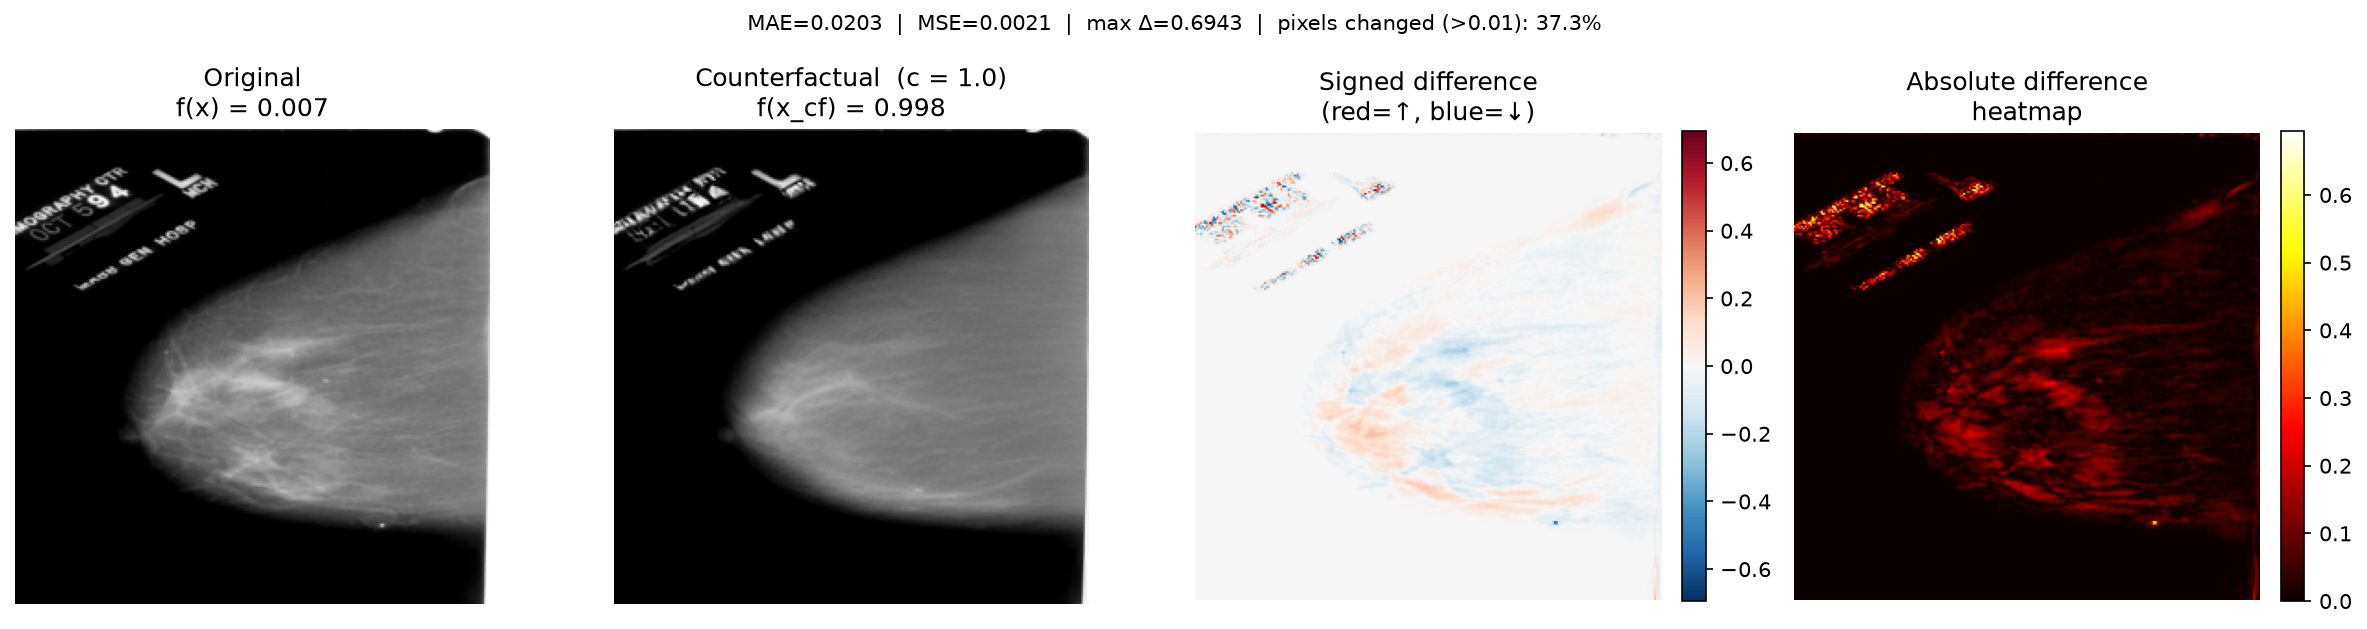
\includegraphics[width=\textwidth]{./checkpoints/cbis_ddsm_breast/counterfactual_diff_n_to_p.png}
  \caption{\textbf{Benign $\to$ malignant}, mammography domain. Same
  four-panel layout as Figures~\ref{fig:n2p}--\ref{fig:p2n}.}
  \label{fig:breast_n2p}
\end{figure}

\begin{figure}[h]
  \centering
  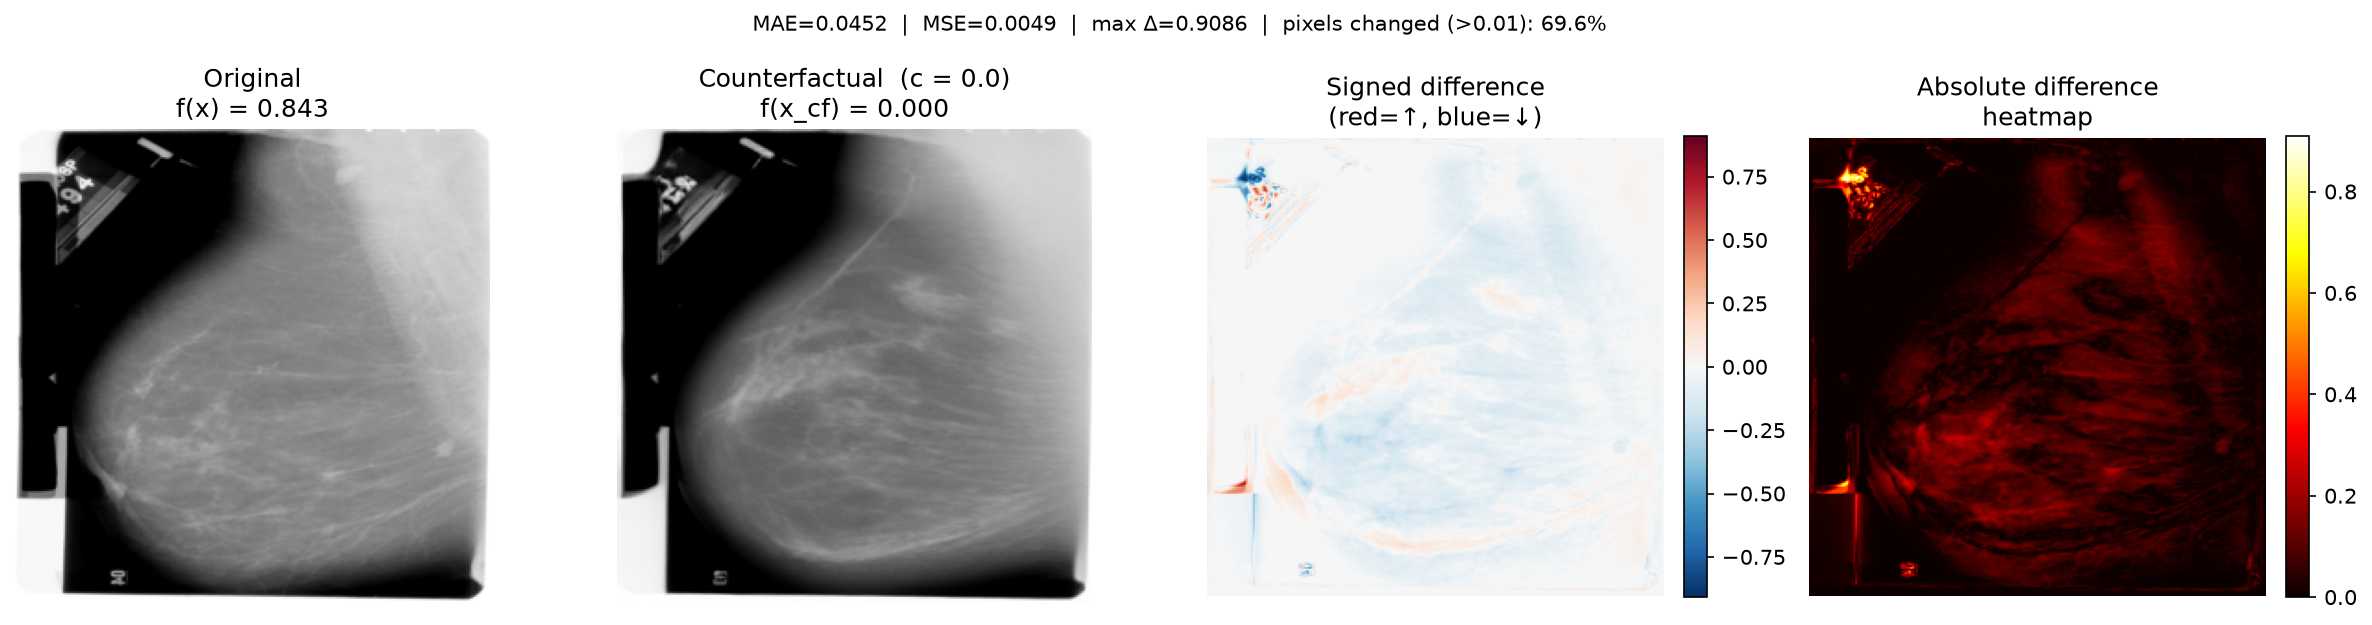
\includegraphics[width=\textwidth]{./checkpoints/cbis_ddsm_breast/counterfactual_diff_p_to_n.png}
  \caption{\textbf{Malignant $\to$ benign}, mammography domain.}
  \label{fig:breast_p2n}
\end{figure}

\textbf{This is not a second validated success, and should not be read as
one.} A mean CV of $1.000$ against the guidance ensemble looks, on its
face, like an even stronger number than the RSNA result; but no
independent held-out re-scoring was run for mammography within the time
available, and the guidance ensemble and the reserved validator backbone
here were all trained on the \emph{same} $\sim$3{,}500-image dataset and
differ only in architecture, so any future held-out check on this domain
would be a weaker, same-corpus test rather than a cross-corpus one. More
tellingly, the metrics that \emph{were} computed already show a
diffuse-edit signature directly, without needing an independent
classifier to surface it: in the malignant$\to$benign direction, BDC
shifts significantly ($p=0.015$) while LLR — the metric that would move
if a lesion actually shrank — does not ($p=0.732$), and edit
concentration (0.33--0.37 against a uniform baseline of $0.05$, with
38--41\% of all pixels changed) is well short of what a focal,
lesion-confined edit would produce. The most defensible reading is that
the classifier is being moved substantially by a diffuse density change
rather than by a change to the segmented lesion itself. What this
extension demonstrates is that the domain-registry architecture
generalizes to a modality sharing essentially nothing with chest
radiography, and that the same purpose-built-diagnostic discipline used
throughout this project catches a plausible adversarial shortcut on a
new domain without requiring a second classifier ensemble to be trained
first; it does not yet demonstrate that the mammography counterfactuals
carry genuine, lesion-specific disease signal, and completing an
independent validator for this domain is the natural next step.

% ═════════════════════════════════════════════════════════════════════════
\section{Conclusion}
% ═════════════════════════════════════════════════════════════════════════

We presented a PPO-controlled, LoRA-fine-tuned latent diffusion pipeline
for generating class-conditional visual counterfactuals on chest
radiographs, with a hard segmentation-mask-gated background lock ensuring
edits stay confined to the lung field. Evaluated with the
Singla~\emph{et al.} protocol plus a model-free identity-preservation
score and two clinical proxy metrics, the system reaches high
counterfactual validity in both edit directions (mean CV $=0.965$) with
statistically significant, directionally sensible shifts in clinical
proxy metrics, while surfacing — and, through two documented reward-bug
fixes, partially correcting — a persistent generative asymmetry between
adding and removing pathology evidence. Head-to-head comparison against a
GAN-based counterfactual baseline and an unguided CycleGAN baseline
(Section~\ref{sec:baseline_comparison}) shows the system matches
GAN-based counterfactual validity while generating substantially more
realistic images. As additional work, we showed the pipeline generalizes
architecturally to a second, dissimilar domain (mammography, CBIS-DDSM,
Section~\ref{sec:breast}), where a purpose-built density diagnostic
surfaced the same diffuse-edit concern found on RSNA; validating those
counterfactuals against an independent classifier, as done here for chest
radiographs, remains open work specific to that domain. A later audit of
the evaluation apparatus itself (Section~\ref{sec:integrity}) closed two
bugs that would have silently invalidated any control-arm or
countermeasure comparison, corrected a set of hand-altered values in the
recorded results, and — on a lesion-annotation metric anchored to ground
truth — showed ensemble guidance to be the one tested countermeasure that
helps, replicated across three seeds, while a Grad-CAM spatial constraint
measurably hurts; a full re-validation of ensemble guidance against
held-out classifiers, at the larger ensemble size the sweep in
Section~\ref{sec:integrity} suggests is worth pursuing, remains the item
that work did not close. The clearest next
steps for the core system are scaling PPO training
compute (particularly for the harder n$\to$p direction), replacing the
SCP and IP proxies with dedicated, purpose-trained detectors if annotated
data becomes available, and increasing FID evaluation sample size for
tighter realism estimates.

% ═════════════════════════════════════════════════════════════════════════
\begin{thebibliography}{9}

\bibitem{singla2022}
S.~Singla, M.~Eslami, M.~Pollack, S.~Wallace, and K.~Batmanghelich.
\textit{Explaining the Black-box Smoothly — A Counterfactual Approach.}
Medical Image Analysis, 2022.

\bibitem{repaint}
A.~Lugmayr, M.~Danelljan, A.~Romero, F.~Yu, R.~Timofte, and L.~Van~Gool.
\textit{RePaint: Inpainting using Denoising Diffusion Probabilistic Models.}
CVPR, 2022.

\bibitem{blended}
O.~Avrahami, D.~Lischinski, and O.~Fried.
\textit{Blended Diffusion for Text-driven Editing of Natural Images.}
CVPR, 2022.

\bibitem{rombach2022}
R.~Rombach, A.~Blattmann, D.~Lorenz, P.~Esser, and B.~Ommer.
\textit{High-Resolution Image Synthesis with Latent Diffusion Models.}
CVPR, 2022.

\bibitem{hu2021lora}
E.~J.~Hu, Y.~Shen, P.~Wallis, Z.~Allen-Zhu, Y.~Li, S.~Wang, L.~Wang, and
W.~Chen.
\textit{LoRA: Low-Rank Adaptation of Large Language Models.}
ICLR, 2022.

\bibitem{schulman2017ppo}
J.~Schulman, F.~Wolski, P.~Dhariwal, A.~Radford, and O.~Klimov.
\textit{Proximal Policy Optimization Algorithms.}
arXiv:1707.06347, 2017.

\bibitem{rsna}
RSNA Pneumonia Detection Challenge, Kaggle, 2018.
\url{https://www.kaggle.com/c/rsna-pneumonia-detection-challenge}

\bibitem{cohen2020xrv}
J.~P.~Cohen, J.~D.~Viviano, P.~Bertin, P.~Morrison, P.~Torabian,
M.~Guarrera, M.~P.~Lungren, A.~Chaudhari, R.~Brooks, M.~Hashir, and
H.~Bertrand.
\textit{TorchXRayVision: A library of chest X-ray datasets and models.}
MIDL, 2022.

\bibitem{lee2017cbisddsm}
R.~S.~Lee, F.~Gimenez, A.~Hoogi, K.~K.~Miyake, M.~Gorovoy, and D.~L.~Rubin.
\textit{A Curated Mammography Data Set for Use in Computer-Aided Detection
and Diagnosis Research.} Scientific Data, vol.~4, 170177, 2017.

\bibitem{ronneberger2015unet}
O.~Ronneberger, P.~Fischer, and T.~Brox.
\textit{U-Net: Convolutional Networks for Biomedical Image Segmentation.}
MICCAI, 2015.

\end{thebibliography}

\end{document}